\documentclass{article}

% NeurIPS 2019 style (course-referenced). Use [final] for a camera-ready copy.
\usepackage[final]{neurips_2019}

% Replace the conference footer with course information.
\makeatletter
\renewcommand{\@noticestring}{MSDM5054 Statistical Machine Learning, Project 1: Mini-Project}
\makeatother

\usepackage[utf8]{inputenc}
\usepackage[T1]{fontenc}
\usepackage{hyperref}
\usepackage{url}
\usepackage{booktabs}
\usepackage{amsfonts}
\usepackage{amsmath}
\usepackage{microtype}
\usepackage{graphicx}
\usepackage{subcaption}
\usepackage{xurl}
\usepackage{tabularx}

\title{Home Credit Default Risk: A Statistical Machine Learning Project}

\author{%
  SHU Yi, CAO Yixin, ZHANG Yajing, SU Zhiyu \\
  MSDM5054 Statistical Machine Learning, Project 1: Mini-Project \\
  Hong Kong University of Science and Technology
}

\begin{document}

\maketitle

\begin{abstract}
This project predicts repayment difficulty in the Kaggle Home Credit Default Risk competition. We compare a V0 baseline pipeline against a revised V1 pipeline built from training-partition exploratory data analysis: \textbf{20} near-constant and \textbf{35} collinear fields are dropped, \textbf{65} original features are retained, and a derived annuity-to-credit ratio is added, so \textbf{66} raw features become \textbf{83} numeric model inputs. A stratified split assigns 246,008 applications to training and 61,503 to development validation. We fit logistic regression, LightGBM and XGBoost, and select \textbf{XGBoost} for its slightly higher five-fold mean ROC-AUC (\textbf{0.767210} versus \textbf{0.766092} for regularized LightGBM) and lower fold variability (\textbf{0.001586} versus \textbf{0.002189}). On the fixed validation set the models are effectively tied: XGBoost AUC \textbf{0.772394}, LightGBM \textbf{0.772396}. The XGBoost Kaggle submission scores \textbf{0.76656} (public) and \textbf{0.76225} (private). Metrics are independently recomputed, and error and calibration analyses focus on XGBoost. Neither the small fixed-set difference nor the five-fold comparison establishes significant superiority.
\end{abstract}

\section{Research questions and data}
This is the Kaggle Home Credit Default Risk competition (\url{https://www.kaggle.com/c/home-credit-default-risk/}): predict from a loan application whether the applicant will have difficulty repaying. The project asks whether application information can rank repayment risk; whether the V1 feature and preprocessing package improves on the V0 baseline; and how ranking performance translates into errors at different classification thresholds. Here V0 denotes the baseline preprocessing and feature pipeline, and V1 its revised version. \texttt{TARGET}=1 denotes the competition's repayment-difficulty class, referred to here as the positive class. Results do not establish causal effects or prescribe lending decisions.

The official labelled application table contains 307,511 rows and the official test table contains 48,744 rows. The experiments use the application main table. ID \texttt{SK\_ID\_CURR} and \texttt{TARGET} are excluded from predictor inputs. The fixed split uses seed 42 and stratification by \texttt{TARGET}. The evaluation dataset contains 61,503 distinct IDs, 4,965 positives and 56,538 negatives.

\section{Data preparation and feature engineering}
Two pipelines are compared: a V0 baseline and a V1 revision, both fitted on the training partition only. V0 replaces the \texttt{DAYS\_EMPLOYED} sentinel 365243 with missing values, applies log1p to four monetary variables, drops features with over 80\% training missingness, and uses numeric imputation/scaling plus categorical one-hot encoding. The logistic classifier is part of a single fitted pipeline.

Our training-partition exploratory data analysis identifies missingness patterns, extreme values, near-constant fields and correlated feature groups. Missingness is informative: applications missing \texttt{EXT\_SOURCE\_1} or \texttt{EXT\_SOURCE\_3} default at higher rates than those with observed values. The V1 decision list drops 20 near-constant fields (a single value in at least 99\% of rows) and 35 collinear fields (Spearman $|r|>0.9$, keeping the highest-information representative per group), retains 65 original features, and adds the annuity-to-credit ratio \texttt{ANNUITY\_TO\_CREDIT}. Among eleven screened ratio features, only \texttt{ANNUITY\_TO\_CREDIT} outperforms both parent columns. Thus 66 raw features become 83 numeric model inputs after additional indicators. V1 changes the preprocessing package as well as feature selection: training-fitted caps and bins, rare-category merging, cross-fitted target encoding for two high-cardinality fields, and ordinal encoding for other categories. Therefore the V0-to-V1 improvement cannot be attributed solely to the single ratio feature. Information value (IV) measures a feature's univariate separation of the two classes across binned values, with larger values indicating stronger separation. IV concentrates sharply on the external credit scores (Table~\ref{tab:iv}, Figure~\ref{fig:iv-ranking}); the removed collinear fields are dominated by correlated building-descriptor blocks. In that table, \texttt{EXT\_SOURCE\_1}--\texttt{EXT\_SOURCE\_3} are external credit scores, \texttt{DAYS\_EMPLOYED} is employment tenure, \texttt{AMT\_GOODS\_PRICE} is the goods price, \texttt{DAYS\_BIRTH} encodes age, and \texttt{OCCUPATION\_TYPE} and \texttt{ORGANIZATION\_TYPE} are occupation and employer categories.

\begin{table}[ht]
\centering
\small
\caption{Information value of the leading features on the training partition.}
\label{tab:iv}
\begin{tabular}{lr}
\toprule
Feature & Information value \\
\midrule
\texttt{EXT\_SOURCE\_3} & 0.330 \\
\texttt{EXT\_SOURCE\_2} & 0.303 \\
\texttt{EXT\_SOURCE\_1} & 0.151 \\
\texttt{DAYS\_EMPLOYED} & 0.112 \\
\texttt{ANNUITY\_TO\_CREDIT} & 0.092 \\
\texttt{AMT\_GOODS\_PRICE} & 0.091 \\
\texttt{DAYS\_BIRTH} & 0.087 \\
\texttt{OCCUPATION\_TYPE} & 0.083 \\
\texttt{ORGANIZATION\_TYPE} & 0.068 \\
\bottomrule
\end{tabular}
\end{table}

\begin{figure}[ht]
  \centering
  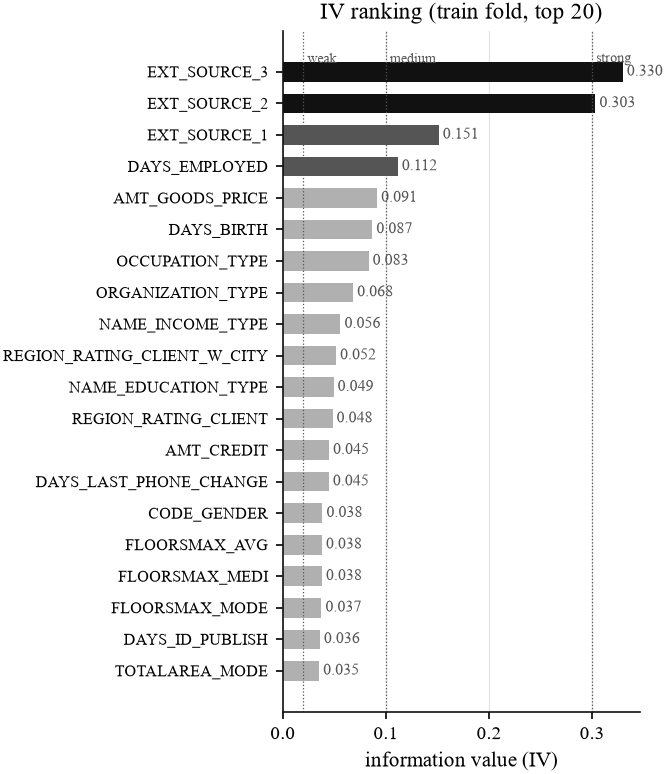
\includegraphics[width=0.55\columnwidth]{../../results/eda/figures/23_iv_ranking.png}
  \caption{Information-value ranking of the leading features on the training partition.}
  \label{fig:iv-ranking}
\end{figure}

\section{Model development and current selection}
We first fit logistic regression and LightGBM, then apply the V1 feature/preprocessing package and regularization. XGBoost uses the same 83-column representation, fixed 80/20 split and five-fold partitioning within the 80\% training portion. Learned preprocessing is fitted within each CV fold.

XGBoost uses binary logistic loss, learning rate 0.03, max depth 6, row and column subsampling 0.8, alpha 0.1, lambda 1.0 and histogram-based trees. Early stopping monitors AUC. Its best CV round counts are 694, 477, 582, 793 and 805; their rounded mean is \textbf{670}. XGBoost is selected because its CV mean is slightly higher and its observed fold variability is lower.

\subsection{Validation models and full-data models}
\begin{table}[ht]
\centering
\small
\caption{Validation models and full-data models.}
\label{tab:models}
\begin{tabularx}{\columnwidth}{@{}l>{\raggedright\arraybackslash}X>{\raggedright\arraybackslash}X@{}}
\toprule
Model & Fixed-validation fitted model & Separate full-data fitted model \\
\midrule
Regularized LightGBM & Validation early stopping selected 892 rounds & 705 rounds selected from CV; 307,511 training rows \\
XGBoost & \texttt{best\_iteration}=777 (zero-based), i.e.\ 778 rounds & 670 rounds selected from CV; 307,511 training rows \\
\bottomrule
\end{tabularx}
\end{table}

Validation metrics are computed from the fixed-validation models; the full-data models are used for the final predictions (Table~\ref{tab:models}). On the Kaggle leaderboard the XGBoost submission \texttt{submission\_v2\_xgboost.csv} scores \textbf{0.76656} (public) and \textbf{0.76225} (private), using the \textbf{V1 feature pipeline}.

\section{Evaluation and input checks}
Our evaluation pipeline reads both models' prediction files, requires 61,503 rows, checks unique nonmissing customer IDs, binary labels and finite probabilities in $[0,1]$, and recomputes AUC. Before comparing models, we join by \texttt{SK\_ID\_CURR}, verify equal ID sets and check that labels agree.

ROC-AUC measures ranking; Average Precision (AP) summarizes precision-recall performance using \texttt{average\_precision\_score}, not trapezoidal PR-AUC. Brier score and log loss measure probability quality. The positive rate is \textbf{8.07\%}: predicting all applications negative gives \textbf{91.93\%} accuracy and zero recall. Thus accuracy alone is misleading.

For XGBoost, a 500-replicate stratified percentile bootstrap (seed 42) yields AUC interval \textbf{[0.7656, 0.7796]}. It conditions on fixed predictions and does not account for model selection, early stopping or training variability. Wilson intervals in calibration plots describe within-bin positive-rate uncertainty only.

\section{Updated model comparison}
\begin{table}[ht]
\centering
\small
\caption{Fixed-validation and cross-validation AUC by experiment.}
\label{tab:comparison}
\begin{tabular}{lrr}
\toprule
Experiment & Fixed validation AUC & CV mean AUC \\
\midrule
V0 Logistic Regression & 0.751239 & --- \\
V0 LightGBM & 0.759364 & --- \\
V1 LightGBM baseline & 0.769522 & 0.763755 \\
V1 Regularized LightGBM & 0.772396 & 0.766092 \\
V1 Regularized + class weight (corrected) & --- & 0.765550 \\
\textbf{V1 XGBoost --- selected model} & \textbf{0.772394} & \textbf{0.767210} \\
\bottomrule
\end{tabular}
\end{table}

The V0 baselines anchor the comparison (Table~\ref{tab:comparison}): logistic regression reaches \textbf{0.751239} and V0 LightGBM \textbf{0.759364}. The V1 feature and preprocessing package lifts LightGBM to \textbf{0.769522} (about $+0.010$), and regularization adds roughly $+0.003$ to \textbf{0.772396}; XGBoost then matches it on the fixed set. The V0-to-V1 gain is thus the larger and more consistent effect. We independently recompute both fixed-validation AUCs. The CV mean difference is \textbf{+0.001118} in favor of XGBoost. Fixed-validation AUC difference (XGBoost minus LightGBM) is \textbf{-0.000002}, effectively a tie. There is no observed improvement in fixed-validation AUC for XGBoost. A class-imbalance-weighted LightGBM variant (per-fold \texttt{scale\_pos\_weight}) reached a CV mean of \textbf{0.765550}, marginally below the unweighted regularized model (\textbf{0.766092}); an earlier weighting run was discarded after stopping in two boosting iterations, and the corrected run reported here restricts early stopping to monitor AUC only.

\subsection{Consistent reporting of fold variability}
\begin{table}[ht]
\centering
\small
\caption{Cross-validation mean and fold standard deviation under two conventions.}
\label{tab:variability}
\begin{tabular}{lrrr}
\toprule
Model & CV mean & Sample SD ($ddof{=}1$) & Population SD ($ddof{=}0$) \\
\midrule
Regularized LightGBM & 0.766092 & 0.002189 & 0.001958 \\
XGBoost & 0.767210 & 0.001586 & 0.001418 \\
\bottomrule
\end{tabular}
\end{table}

The XGBoost calculation uses \texttt{np.std} with its default \texttt{ddof=0}, while LightGBM uses \texttt{ddof=1}; both standard deviations are recomputed here under a common convention (Table~\ref{tab:variability}). XGBoost still has lower observed fold variability after harmonization (Figure~\ref{fig:cv}). These SDs are not standard errors or confidence intervals, and no significance claim is made from five folds.

\begin{figure}[ht]
  \centering
  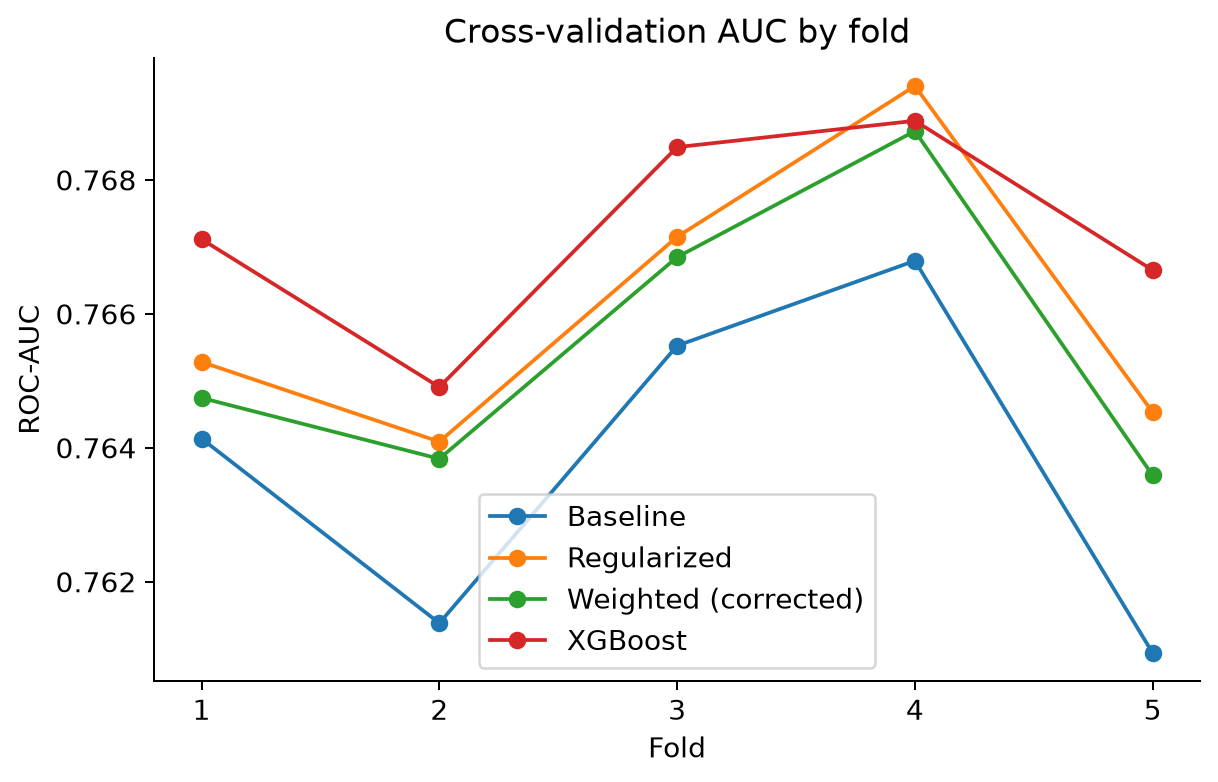
\includegraphics[width=0.7\columnwidth]{../../results/evaluation/figures/07_cv_comparison.png}
  \caption{Cross-validation AUC comparison across folds.}
  \label{fig:cv}
\end{figure}

\section{Independently recomputed fixed-validation metrics}
\begin{table}[ht]
\centering
\small
\caption{Metrics recomputed from aligned prediction files.}
\label{tab:metrics}
\begin{tabular}{lrr}
\toprule
Metric & Regularized LightGBM & XGBoost \\
\midrule
ROC-AUC $\uparrow$ & 0.772396 & 0.772394 \\
Average precision $\uparrow$ & 0.262523 & 0.261932 \\
Brier score $\downarrow$ & 0.066919 & 0.066902 \\
Log loss $\downarrow$ & 0.241821 & 0.241746 \\
\bottomrule
\end{tabular}
\end{table}

The models are very similar (Table~\ref{tab:metrics}). XGBoost has slightly lower probability losses, while LightGBM has slightly higher AP and essentially identical AUC. The data do not support a claim that one model dominates all metrics. Our model-selection preference is driven primarily by CV. The aligned ROC and PR curves (Figure~\ref{fig:comparison}) use the same 61,503 applications.

\begin{figure*}[!t]
  \centering
  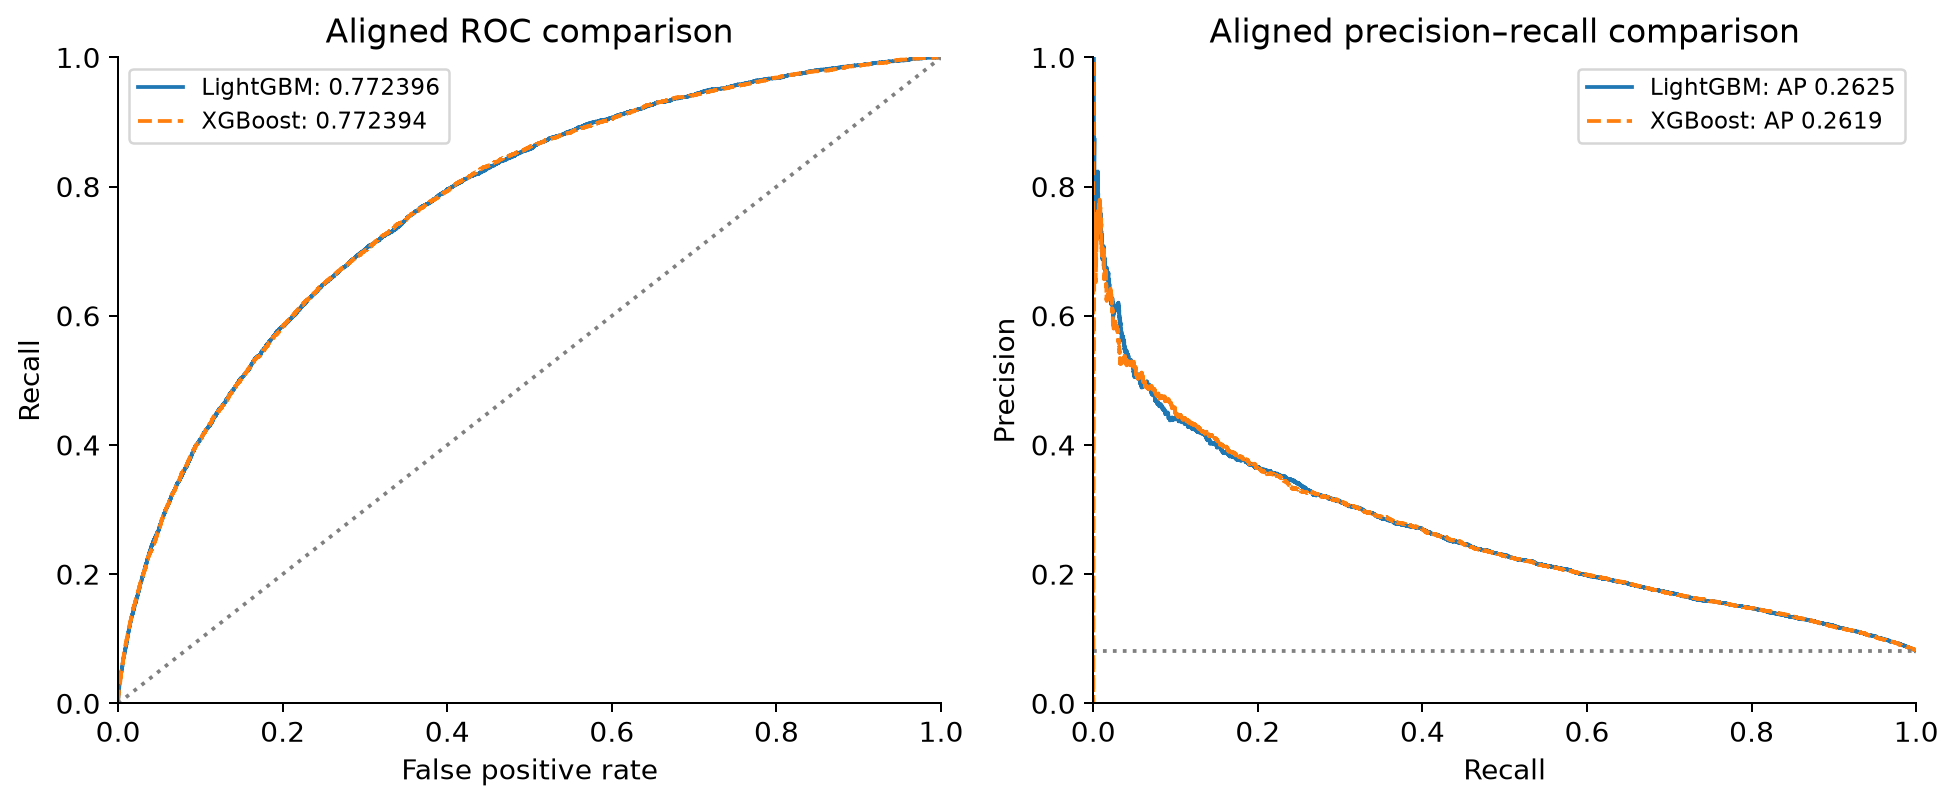
\includegraphics[width=0.8\textwidth]{../../results/evaluation/figures/10_model_comparison.png}
  \caption{Aligned ROC and precision-recall comparison of the two models.}
  \label{fig:comparison}
\end{figure*}

The following plots (Figure~\ref{fig:rocpr} and Figure~\ref{fig:calibration}) and sections focus on the selected \textbf{XGBoost} model.

\begin{figure}[ht]
  \centering
  \begin{subfigure}[b]{0.48\columnwidth}
    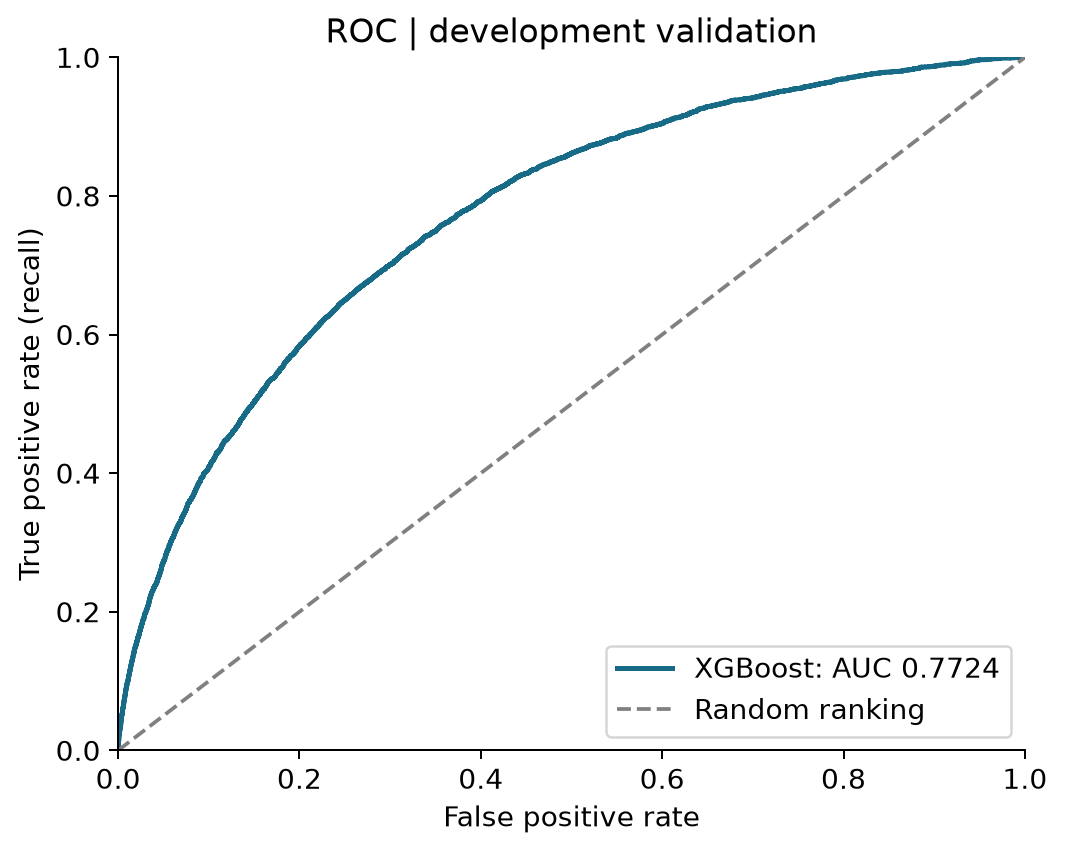
\includegraphics[width=\columnwidth]{../../results/evaluation/figures/01_roc.png}
    \caption{ROC curve}
  \end{subfigure}\hfill
  \begin{subfigure}[b]{0.48\columnwidth}
    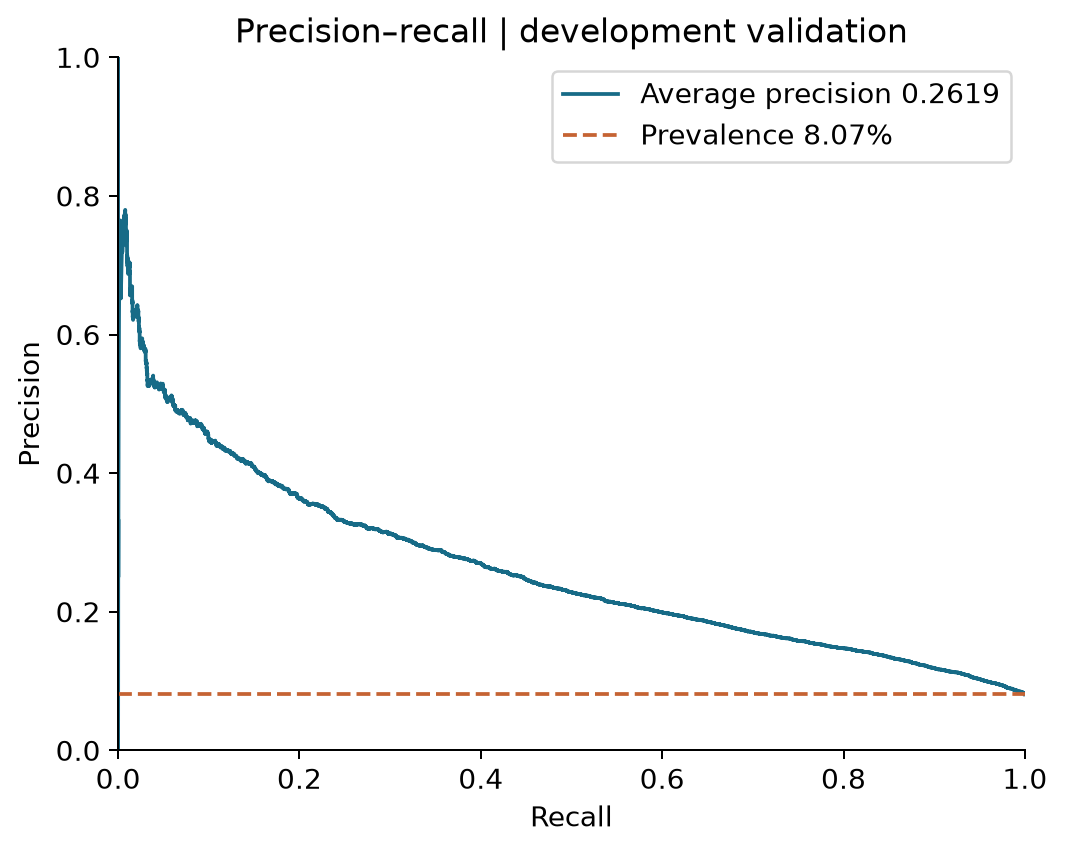
\includegraphics[width=\columnwidth]{../../results/evaluation/figures/02_precision_recall.png}
    \caption{Precision-recall curve}
  \end{subfigure}
  \caption{XGBoost ROC and precision-recall curves.}
  \label{fig:rocpr}
\end{figure}

\begin{figure}[ht]
  \centering
  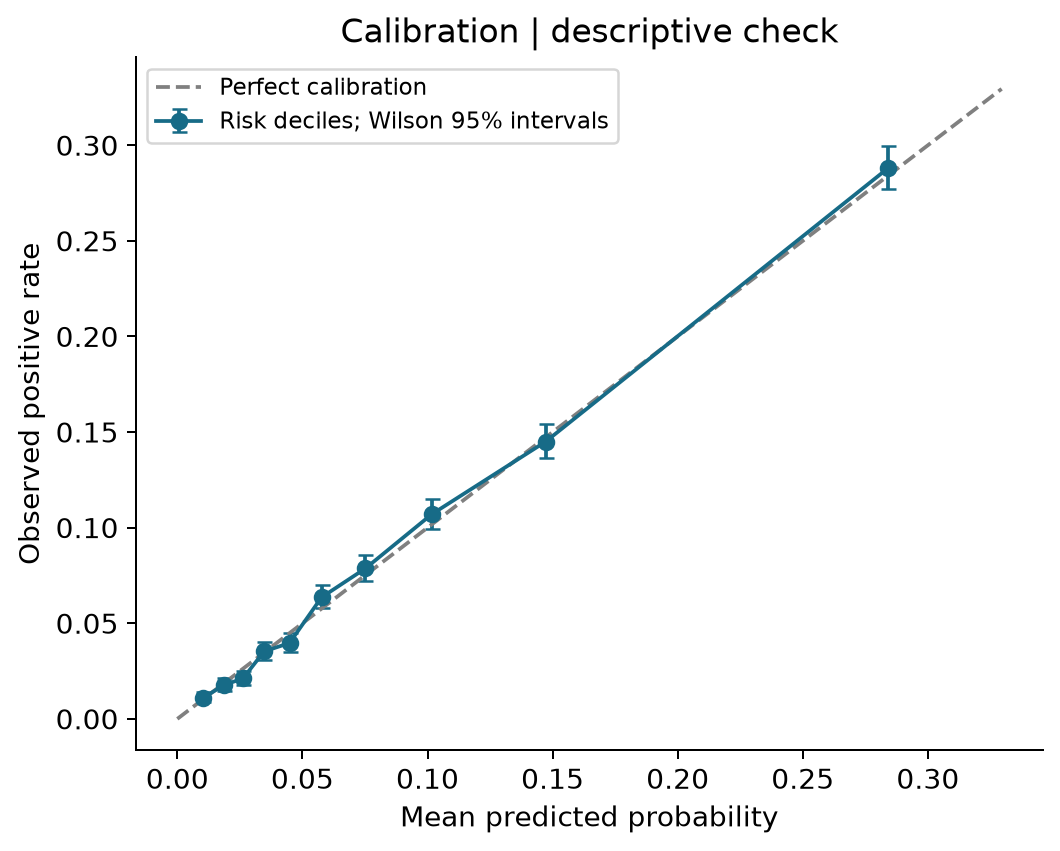
\includegraphics[width=0.6\columnwidth]{../../results/evaluation/figures/05_calibration.png}
  \caption{XGBoost calibration plot.}
  \label{fig:calibration}
\end{figure}

XGBoost mean predicted risk is 8.0070\%, versus observed prevalence 8.0728\%. Its Brier score 0.066902 is below the descriptive constant-validation-prevalence reference 0.074211. That reference is not a separately trained model. Similar average predicted and observed risk does not establish calibration for every score range or subgroup.

\section{XGBoost thresholds and error analysis}
Thresholds are prespecified illustrative comparisons, not optimized business decisions. Predict class 1 when probability is greater than or equal to the threshold.

\begin{table}[ht]
\centering
\small
\caption{Confusion-matrix summary at illustrative thresholds.}
\label{tab:thresholds}
\begin{tabular}{lrrrrrr}
\toprule
Threshold & True positive & False positive & False negative & Precision & Recall & Fraction flagged \\
\midrule
0.05 & 4,209 & 26,876 & 756 & 13.54\% & 84.77\% & 50.54\% \\
0.10 & 3,041 & 12,474 & 1,924 & 19.60\% & 61.25\% & 25.23\% \\
0.15 & 2,198 & 6,544 & 2,767 & 25.14\% & 44.27\% & 14.21\% \\
0.20 & 1,590 & 3,659 & 3,375 & 30.29\% & 32.02\% & 8.53\% \\
0.30 & 798 & 1,215 & 4,167 & 39.64\% & 16.07\% & 3.27\% \\
0.50 & 143 & 105 & 4,822 & 57.66\% & 2.88\% & 0.40\% \\
\bottomrule
\end{tabular}
\end{table}

Table~\ref{tab:thresholds} reports the confusion metrics at all six thresholds. At 0.50, XGBoost flags \textbf{248} applications and detects only \textbf{143 / 4,965} positives (recall \textbf{2.88\%}); it misses \textbf{4,822} positives despite accuracy \textbf{91.99\%} (Figure~\ref{fig:confusion}). At 0.10, recall rises to \textbf{61.25\%}, with \textbf{12,474} false positives and precision \textbf{19.60\%}. Lowering the threshold from 0.50 to 0.10 raises recall from \textbf{2.88\%} to \textbf{61.25\%} while false positives rise from \textbf{105} to \textbf{12,474} (Figure~\ref{fig:tradeoffs}); this is a trade-off, not an unconditional improvement.

\begin{figure*}[!t]
  \centering
  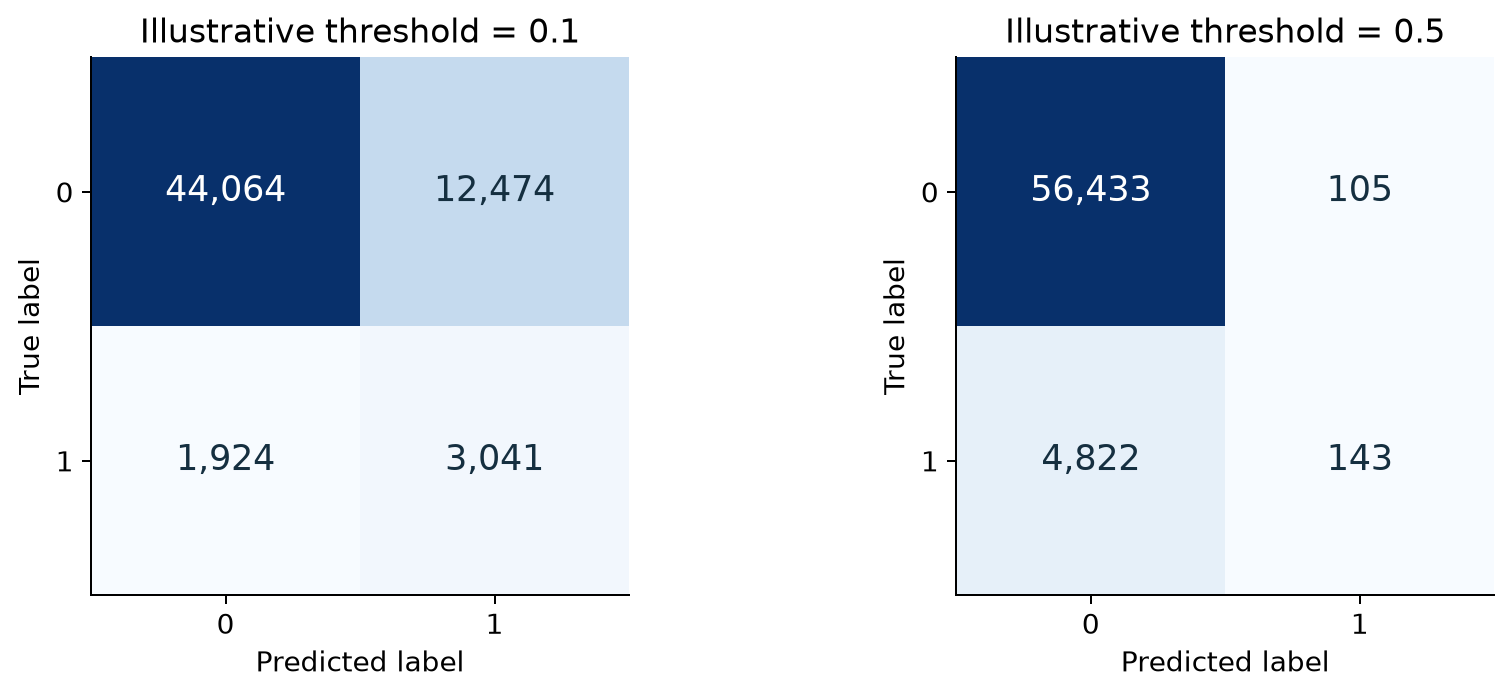
\includegraphics[width=0.8\textwidth]{../../results/evaluation/figures/03_confusion_matrices.png}
  \caption{XGBoost confusion matrices at illustrative thresholds.}
  \label{fig:confusion}
\end{figure*}

\begin{figure}[ht]
  \centering
  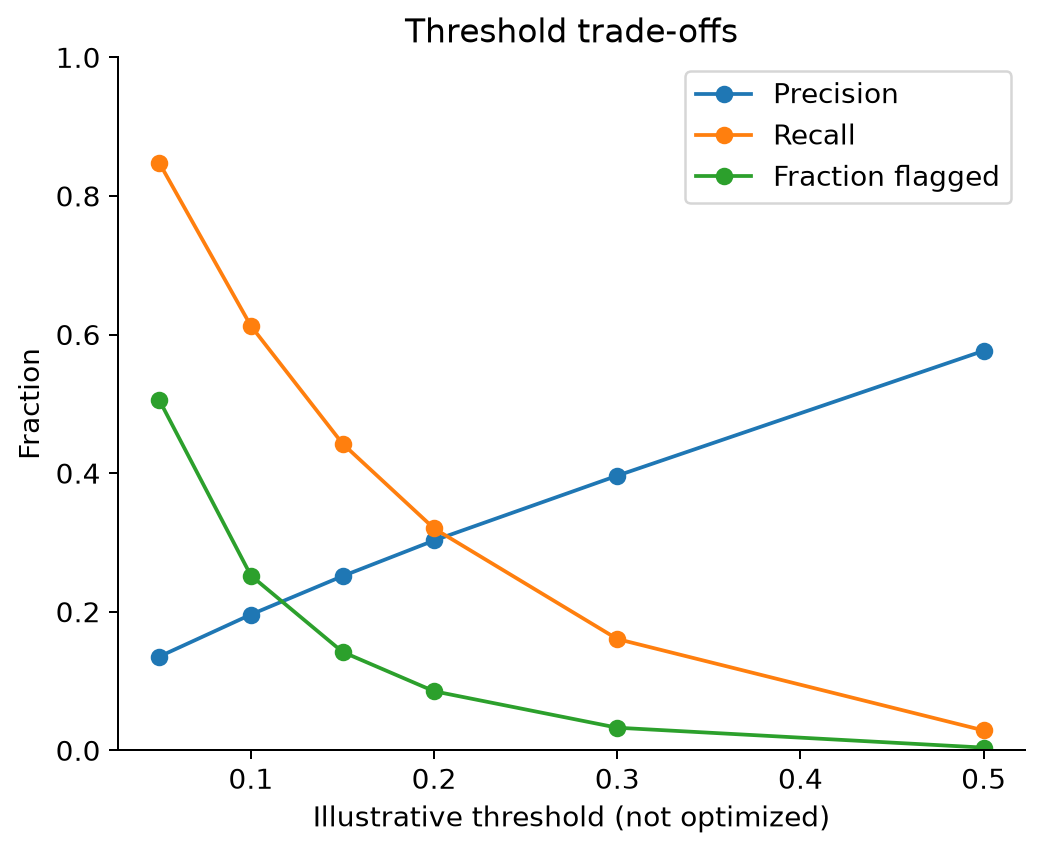
\includegraphics[width=0.6\columnwidth]{../../results/evaluation/figures/04_threshold_tradeoffs.png}
  \caption{Threshold trade-off curves.}
  \label{fig:tradeoffs}
\end{figure}

\begin{figure}[ht]
  \centering
  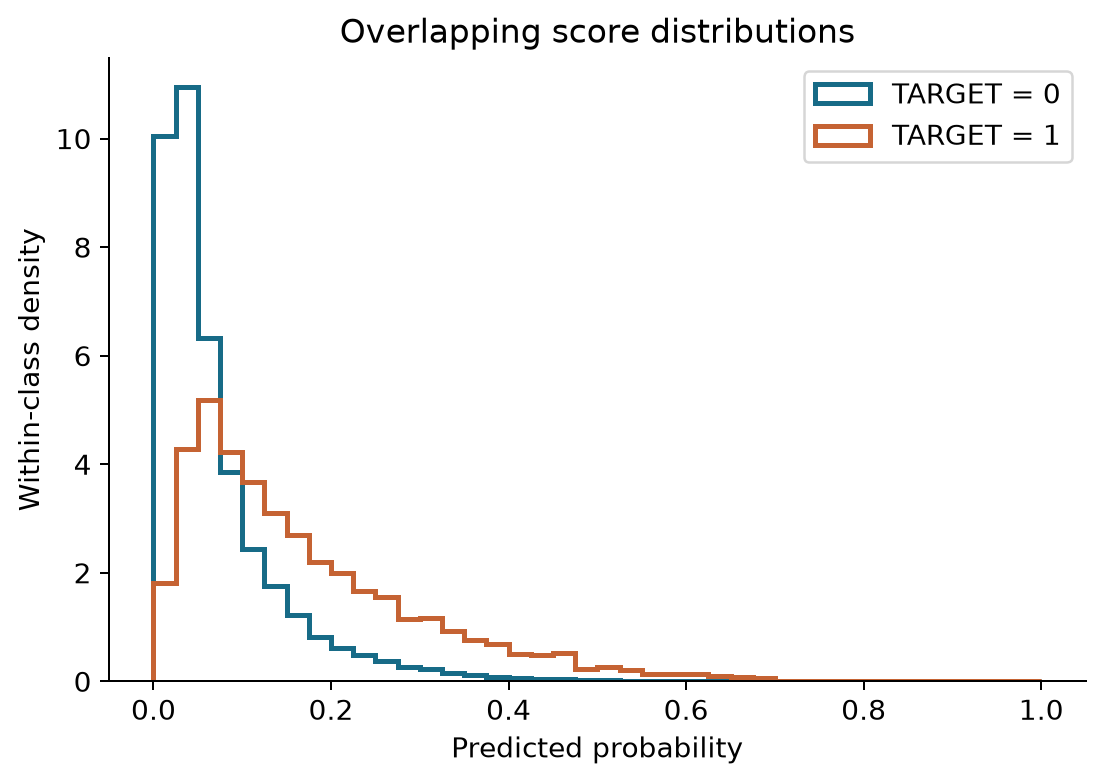
\includegraphics[width=0.6\columnwidth]{../../results/evaluation/figures/09_score_distributions.png}
  \caption{Predicted-score distributions for errors at threshold 0.10.}
  \label{fig:scores}
\end{figure}

At threshold 0.10, XGBoost false negatives have median predicted probability 0.0583 and false positives 0.1539. Overlapping score distributions (Figure~\ref{fig:scores}) explain why lowering the threshold increases detection and false alarms together. Available inputs support score-based error analysis, but not claims about age-, income- or occupation-specific mistakes. A future operational threshold requires explicit costs or capacity, selected using training-side out-of-fold predictions and assessed on fresh data.

\section{XGBoost risk concentration and feature interpretation}
The highest-risk decile contains \textbf{6,151} applications and \textbf{1,772} positives. Its positive rate is \textbf{28.81\%}, about \textbf{3.57 times} the overall rate; it contains \textbf{35.69\%} of all positives. The lowest-risk decile's positive rate is \textbf{1.11\%}. Quantile bins are descriptive groupings of these validation predictions, not frozen production cutoffs (Figure~\ref{fig:deciles-importance}).

The XGBoost normalized gain importance (from the full-data model) is led by the external credit-score features \texttt{EXT\_SOURCE\_2}, \texttt{EXT\_SOURCE\_3} and \texttt{EXT\_SOURCE\_1}, followed by \texttt{NAME\_EDUCATION\_TYPE} (education level) and \texttt{FLAG\_OWN\_CAR} (car ownership) (Figure~\ref{fig:deciles-importance}). It does not provide the direction of effects and is not SHAP or causal evidence.

\begin{figure}[ht]
  \centering
  \begin{subfigure}[b]{0.48\columnwidth}
    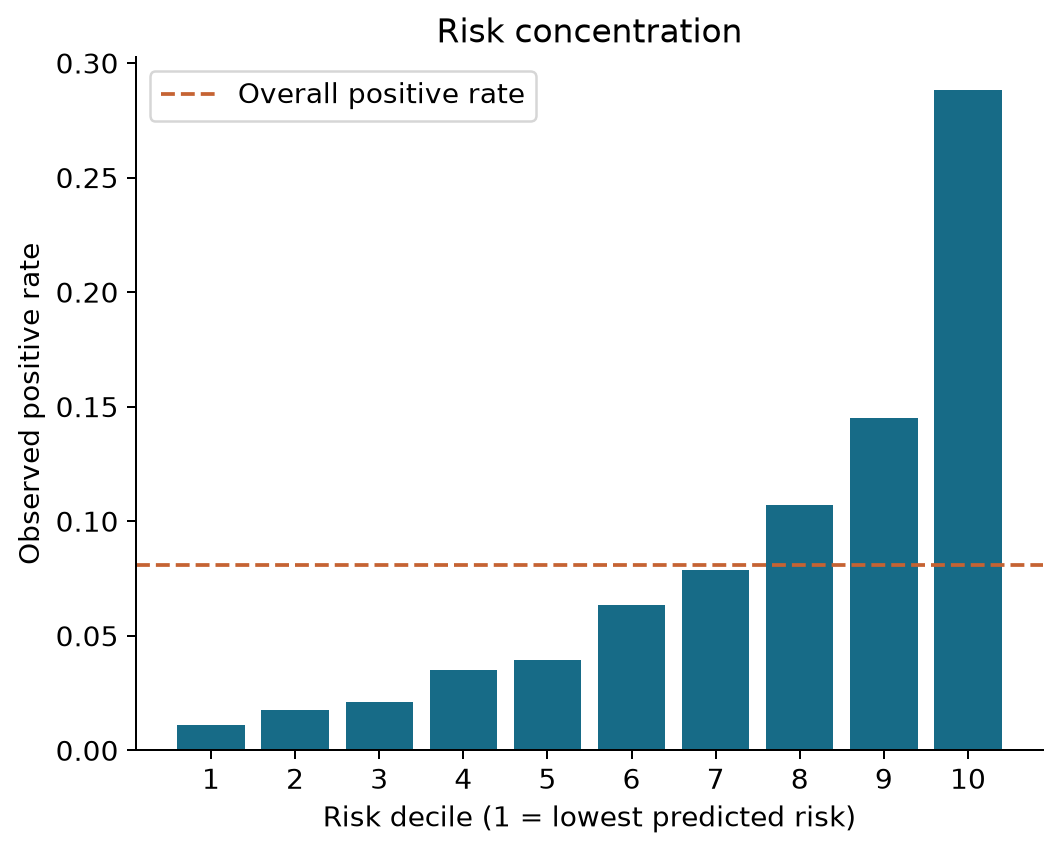
\includegraphics[width=\columnwidth]{../../results/evaluation/figures/06_risk_deciles.png}
    \caption{Risk deciles}
  \end{subfigure}\hfill
  \begin{subfigure}[b]{0.48\columnwidth}
    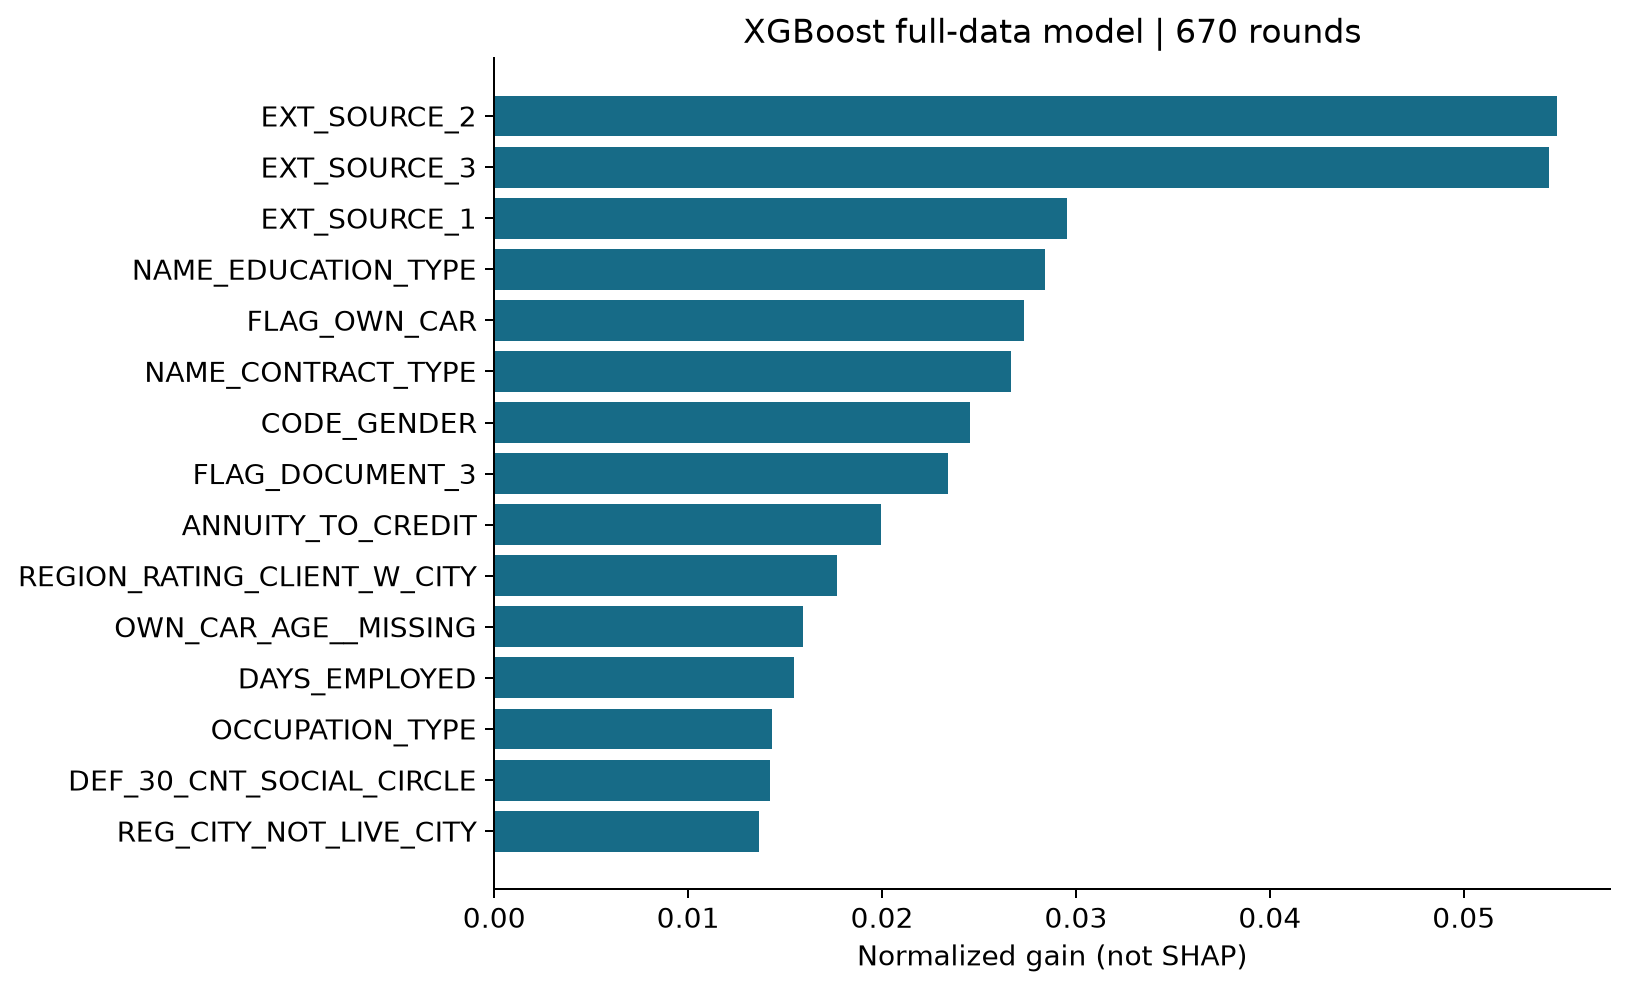
\includegraphics[width=\columnwidth]{../../results/evaluation/figures/08_feature_importance.png}
    \caption{Feature importance}
  \end{subfigure}
  \caption{XGBoost risk deciles and full-data feature importance.}
  \label{fig:deciles-importance}
\end{figure}

\section{Limitations and next steps}
\begin{enumerate}
\item Both fixed-validation models used the same evaluation set for early stopping. Neither result is an unbiased untouched-test estimate.
\item Feature selection precedes inner CV, so the whole feature-selection process is not nested.
\item No paired significance test is reported, and earlier logistic and V0 models are not included in the aligned comparison.
\item Feature-based subgroup errors, temporal generalization and fairness evaluation remain outside this analysis.
\item SHAP explanations are not computed for the evaluated estimator.
\end{enumerate}

\section{Conclusions}
We select XGBoost for the current V1 pipeline because it has a modestly higher mean five-fold AUC and lower observed fold variability under a common SD convention. Fixed-validation ranking is practically unchanged relative to regularized LightGBM, and probability/precision-recall differences are small and mixed. The recomputed metrics, aligned comparison curves and XGBoost-focused error analysis support that nuanced conclusion. A default threshold of 0.50 remains ineffective for positive detection. Stronger generalization or deployment claims require fresh evaluation and explicit operating objectives.

\section{Use of AI and large language models}
AI and large language models were used throughout the project as drafting and debugging assistants. They helped scaffold the Python data, modeling and evaluation code, draft and iteratively refine this report and its tables, and check numerical consistency across sections. All AI-generated code was executed and tested by the team, and every reported number was verified against the exported artifacts. Scientific decisions and final wording were reviewed and approved by the team members.

\section{Contributions and evidence}
\begin{table}[ht]
\centering
\small
\begin{tabularx}{\columnwidth}{@{}l>{\raggedright\arraybackslash}X@{}}
\toprule
Member & Contribution \\
\midrule
SHU Yi & Data entry, fixed split, shared V0 pipeline and submission validation \\
CAO Yixin & Training-partition EDA, feature decisions, analysis figures, Kaggle submission, and NeurIPS-format report conversion and reorganization \\
ZHANG Yajing & LightGBM and XGBoost, CV/tuning, model selection, full-data fitting and prediction generation \\
SU Zhiyu & Recomputed metrics, ID-aligned comparison, harmonized CV variability, error analysis, figures and integrated report \\
\bottomrule
\end{tabularx}
\end{table}

Source code and notebooks are available at \url{https://github.com/slowdowndown/msdm5054-home-credit}.

\end{document}
